\documentclass{howto}
% \usepackage{distutils}
\usepackage{palatino}
\renewcommand{\ttdefault}{cmtt}
\renewcommand{\sfdefault}{cmss}
\newcommand{\myhdl}{\protect \mbox{MyHDL}}
\usepackage{graphicx}
% $Id$

\title{What's New in \myhdl\ 0.3}
\release{0.3}
\author{Jan Decaluwe}
\authoraddress{\email{jan@jandecaluwe.com}}

\begin{document}
\maketitle
\tableofcontents


\section{VCD output for waveform viewing\label{section-wave}}

\ifpdf
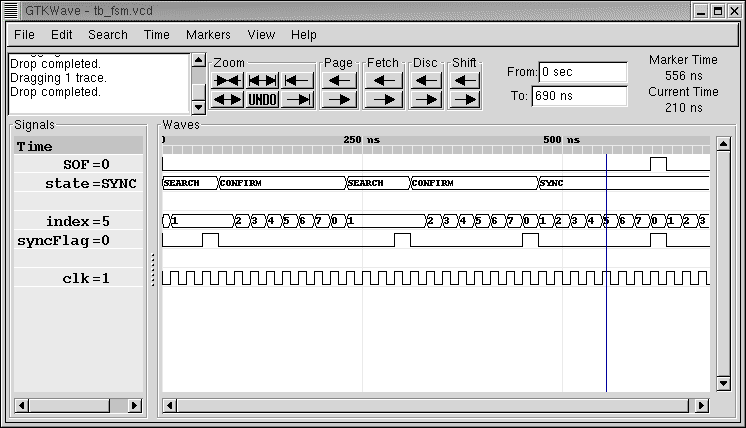
\includegraphics{tbfsm.png}
\fi

\myhdl\ now has support for waveform viewing. During simulation, signal
changes can be written to a VCD output file that can be loaded
into a waveform viewer tool such as \program{gtkwave}.

The user interface of this feature consists of a single function,
\function{traceSignals()}.  To explain how it works, recall that in
\myhdl{}, an instance is created by assigning
the result of a function call to an instance name. For example:

\begin{verbatim}
tb_fsm = testbench()
\end{verbatim}

To enable VCD tracing, the instance should be created as follows
instead:

\begin{verbatim}
tb_fsm = traceSignals(testbench)
\end{verbatim}

All signals in the instance hierarchy will be traced in a VCD
file called \file{tb_fsm.vcd}. Note that first the argument of
\function{traceSignals()} consists of the uncalled function. By
calling the function under its control, \function{traceSignals()}
gathers information about the hierarchy and the signals to be traced.
In addition to a function argument, \function{traceSignals()} accepts
an arbitrary number of non-keyword and keyword arguments that will be
passed to the function call.

Signals are dumped in a suitable format. This format is inferred at
the \class{Signal} construction time, from the type of the initial
value. In particular, \class{bool} signals are dumped as single
bits. (This only works starting with Python~2.3, when \class{bool} has
become a separate type).  Likewise, \class{intbv} signals with a
defined bit width are dumped as bit vectors. To support the general
case, other types of signals are dumped as a string representation, as
returned by the standard \function{str()} function.

\begin{notice}[warning]
Support for literal string representations is not part of the VCD
standard. It is specific to \program{gtkwave}. To generate a
standard VCD file, you need to use signals with a defined bit width
only.
\end{notice}

\section{Enumeration types\label{section-enum}}

It is often desirable to define a set of identifiers.  A standard
Python idiom for this purpose is to assign a range of integers to a
tuple of identifiers, like so:

\begin{verbatim}
>>> SEARCH, CONFIRM, SYNC = range(3)
>>> CONFIRM
1
\end{verbatim}

However, this technique has some drawbacks. Though it is clearly
the intention that the identifiers belong together, this information
is lost as soon as they are defined. Also, the identifiers evaluate to
integers, whereas a string representation of the identifiers
would be preferable. To solve these issues, we need an
\emph{enumeration type}.

\myhdl\ 0.3 supports enumeration types by providing a function
\function{enum()}.  The arguments to \function{enum()} are the string
representations of the identifiers, and its return value is an
enumeration type. The identifiers are available as attributes of the
type. For example:

\begin{verbatim}
>>> from myhdl import enum
>>> t_State = enum('SEARCH', 'CONFIRM', 'SYNC')
>>> t_State
<Enum: SEARCH, CONFIRM, SYNC>
>>> t_State.CONFIRM
CONFIRM
\end{verbatim}

Enumeration types are often used for the state variable in a finite
state machine.  In the waveform in Section~\ref{section-wave}, you see
a \class{Signal} called \var{state}. Note how the waveforms show the
string representation of the enumeration type identifiers The
\var{state} signal has been constructed with an enumeration type
identifier as its initial value, as follows:

\begin{verbatim}
state = Signal(t_State.SEARCH)
\end{verbatim}

\section{Inferring the sensitivity list for combinatorial
logic\label{section-combinatorial}}

In \myhdl{}, combinatorial logic is described by a generator function with
a sensitivity list that contains all inputs signals (the signals that
are read inside the function).

It may be easy to forget some input signals, especially it there are a
lot of them or if the code is being modified. There are various ways
to solve this. One way is to use a sophisticated editor. Another way
is direct language support. For example, recent versions of Verilog
have the \code{always~@*} construct, that infers all input
signals. The SystemVerilog 3.1 standard improves on this by
introducing the \code{always_comb} block with slightly enhanced
semantics.

\myhdl{}~0.3 provides a function called \function{always_comb()} which
is named and modeled after the SystemVerilog counterpart.
\function{always_comb()} takes a classic local function as its
argument. This function should specify the combinatorial logic behavior.
\function{always_comb()} returns a generator
that is sensitive to all inputs, and that will run the function
whenever an input changes.

For example, suppose that we have a mux module described as follows:

\begin{verbatim}
def mux(z, a, b, sel):
    """ Multiplexer.
    
    z -- mux output
    a, b -- data inputs
    sel -- control input

    """
    def logic()
        while 1:
            yield a, b, sel
            if sel == 1:
                z.next = a
            else:
                z.next = b
    mux_logic = logic()
    return mux_logic
\end{verbatim}

Using \function{always_comb()}, we can describe it as follows instead:

\begin{verbatim}
def mux(z, a, b, sel):
    """ Multiplexer.
    
    z -- mux output
    a, b -- data inputs
    sel -- control input

    """
    def logic()
        if sel == 1:
            z.next = a
        else:
            z.next = b
    mux_logic = always_comb(logic)
    return mux_logic
\end{verbatim}

Note that in the first version, the sensitivity list is at the beginning of
the generator function code. This is traditionally done in
synthesizable RTL style modeling. However, the semantics of this style
are not entirely correct: at the start of the simulation, the
combinatorial output will not reflect the initial state of the
inputs. \function{always_comb()} solves this by putting the sensitivity
list at the end of the code.

\section{Inferring the list of instances\label{section-instances}}

In \myhdl{}, the instances defined in a top level function
need to be returned explicitly. The following is a schematic
example:

\begin{verbatim}
def top(...):
    ...
    instance_1 = module_1(...)
    instance_2 = module_2(...)
    ...
    instance_n = module_n(...)
    ... 
    return instance_1, instance_2, ... , instance_n
\end{verbatim}


It may be convenient to assemble the list of instances automatically,
especially if there are many instances. For this purpose,
\myhdl{}~0.3 provides the  function \function{instances()}.
It is used as follows:

\begin{verbatim}
from myhdl import instances

def top(...):
    ...
    instance_1 = module_1(...)
    instance_2 = module_2(...)
    ...
    instance_n = module_n(...)
    ...
    return instances()
\end{verbatim}

Function \function{instances()} uses introspection to inspect the type
of the local variables defined by the calling function. All variables
that comply with the definition of an instance are assembled in
a list, and that list is returned.

\section{Inferring the list of processes\label{section-processes}}

In addition to instances, a top level function may
also define local generators functions, which I will
call \emph{processes} because of the analogy with VHDL.
Like instances, processes need to be returned explicitly,
with the qualification that they have to be called first
to turn them into generators. The following is a schematic
example:

\begin{verbatim}
def top(...):
    ...
    def process_1():
        ...
    def process_2():
        ...
    ...
    def process_n():
        ...
    ...
    return process_1(), process_2(), ..., process_n()
\end{verbatim}

As for instances, it may be more convenient to assemble the list of
processes automatically. One option is to turn each process into an
instance by calling it and assigning the returned generator to a local
variable. Those instances will then be found by the
\function{instances()} function described in
Section~\ref{section-instances}.

Another option is to use the function \function{processes()} provided
by \myhdl{}~0.3 . This function uses introspection to find the
processes, calls each of them, and assembles the returned generators
into a list. It can be used as follows:

\begin{verbatim}
from myhdl import processes

def top(...):
    ...
    def process_1():
        ...
    def process_2():
        ...
    ...
    def process_n():
        ...
    ... 
    return processes()
\end{verbatim}

To conclude, a top level function with both instances and processes
can use the following idiomatic code to return all of them:

\begin{verbatim}
return instances(), processes()
\end{verbatim}

\section{Class \class{intbv} enhancements\label{section-intbv}}

Class \class{intbv} has been enhanced with new features.

It is now possible to leave the left index of a slicing operation
unspecified. The meaning is to access ``all'' higher order bits. For
example:

\begin{verbatim}
>>> from myhdl import intbv
>>> n = intbv()
>>> hex(n)
'0x0'
>>> n[:] = 0xde
>>> hex(n)
'0xde'
>>> n[:8] = 0xfa
>>> hex(n)
'0xfade'
>>> n[8:] = 0xb4
>>> hex(n)
'0xfab4'
\end{verbatim}

\class{intbv} objects now have \var{min} and \var{max} attributes
that can be specified at construction time. The meaning is that
only values within \code{range(min, max)} are permitted. The default
value for these attributes is \var{None}, meaning ``infinite''. For
example (traceback output shortened for clarity):

\begin{verbatim}
>>> n = intbv(min=-17, max=53)
>>> n
intbv(0)
>>> n.min
-17
>>> n.max
53
>>> n[:] = 28
>>> n
intbv(28)
>>> n[:] = -18
Traceback (most recent call last):
    ....
ValueError: intbv value -18 < minimum -17
>>> n[:] = 53
Traceback (most recent call last):
    ....
ValueError: intbv value 53 >= maximum 53
\end{verbatim}

When a slice is taken from an \class{intbv} object, the return value
is a new \class{intbv} object with a defined bit width. As in
Verilog, the value of the new \class{intbv} object is always
positive, regardless of the sign of the original value. In addition,
the \var{min} and \var{max} attributes are set implicitly:

\begin{verbatim}
>>> v = intbv()[6:]
>>> v
intbv(0)
>>> v.min
0
>>> v.max
64
\end{verbatim}

Lastly, a small change was implemented with regard to 
binary operations. In previous versions, both numeric
and bit-wise operations always returned a new \class{intbv}
object, even in mixed-mode operations with \class{int}
objects. This has changed: numeric operations 
return an \class{int}, and bitwise operations return
a \class{intbv}. In this way, the return value corresponds
better to the nature of the operation.

\section{Function \function{concat()} \label{section-concat}}

In previous versions, the \class{intbv} class provided a
\method{concat()} method.  This method is no longer
available. Instead, there is now a \function{concat()} function 
that supports a much broader range of objects.

A function is more natural because \myhdl\ objects of various types
can be concatenated: \class{intbv} objects with a defined bit width,
\class{bool} objects, the corresponding signal objects, and bit
strings. All these objects have a defined bit width.  Moreover, the
first argument doesn't need to have a defined bit width. It can also be
an unsized \class{intbv}, an \class{int}, a \class{long}, or a
corresponding signal object.  Function \function{concat()} returns an
\class{intbv} object.


\section{Python 2.3 support\label{section-Python}}

Python~2.3 was released on July 29, 2003, and as of this writing, it
is the latest stable Python release.  \myhdl{}~0.3 works with both
Python~2.2 and Python~2.3. In good Python tradition, \myhdl\ code
developed with Python~2.2 should run without changes or problems in
Python~2.3.

In general, I am not that keen on early upgrading. However, as it
happens, the evolution of Python enables features that are really
important or even crucial to \myhdl{}.  Python~2.2 generators are the
best example: they are the cornerstone of \myhdl{}. But Python~2.3
also has significant benefits, which I will summarize below.

First, generators and the \code{yield} statement are a default 
Python~2.3 feature. This means that \code{from __future__ import generators}
statements are no longer required.

Second, Python~2.3 has a \class{bool} type, which is implemented as a
subtype of \class{int}. For general Python use, the implications are
rather limited - the main difference is that logical result values
will print as \code{False} and \code{True} instead of \code{0} and
\code{1}. However, in \myhdl{}, I can use the \class{bool} type to
infer a bit width.  If a \class{Signal} is constructed with a
\class{bool} value, it is a single bit \class{Signal}. One application
is waveform viewing as in Section~\ref{section-wave}. In the waveform,
note how single bit signals are displayed as level changes.  With
Python 2.2, the waveforms of these signals would only show value
changes, which is not as clear for single bits.

Finally, Python~2.3 is significantly faster. \myhdl\ code runs
25--35\% faster in Python~2.3. This is a very nice speedup compared to
the small burden of a straightforward upgrade.

Python is a very stable language, so upgrading to Python~2.3 is
virtually risk free. Given the additional benefits, I recommend
\myhdl\ users to do so as soon as possible. For the next major \myhdl\
release, the new features will become required and only Python~2.3
(and higher) will be supported.


\end{document}
